\documentclass[runningheads]{llncs}

\usepackage{listings}
\usepackage{enumitem}
%
\usepackage[T1]{fontenc}

\usepackage{graphicx}
% Used for displaying a sample figure. If possible, figure files should
% be included in EPS format.
%
% If you use the hyperref package, please uncomment the following two lines
% to display URLs in blue roman font according to Springer's eBook style:
%\usepackage{color}
%\renewcommand\UrlFont{\color{blue}\rmfamily}
%
\begin{document}
%
\title{Formalization and Runtime Verification of Invariants for
Robotic Systems}
%
%\titlerunning{Abbreviated paper title}
% If the paper title is too long for the running head, you can set
% an abbreviated paper title here
%
\author{Ricardo Cordeiro\inst{1} \and
Paulo Canelas\inst{1,2} \and
Alcides Fonseca\inst{1} \and
Christopher S. Timperley\inst{2}}
%\orcidID{0000-0002-8959-1702}
%
\authorrunning{Ricardo Cordeiro et al.}
% First names are abbreviated in the running head.
% If there are more than two authors, 'et al.' is used.
%
\institute{Faculdade de Ciências da Universidade de Lisboa,
Lisboa, Portugal \and
Carnegie Mellon University, Pittsburgh, PA}
%
\maketitle              % typeset the header of the contribution
%
\begin{abstract}
    Robotic systems are critical in today's society. A potential failure in a robot may have extraordinary costs, not only financial, but can also cost lives.
    Current practices in robot testing are vast and involve methods like simulation, log checking, or field testing. However, current practices often require human monitoring to determine the correctness of a given behavior. Automating this analysis can not only relieve the burden from a high-skilled engineer, but also allow for massive parallel executions of tests, that can detect behavioral faults in the robots that would otherwise not be found due to human error or lack of time.
    We have developed a DSL (domain-specific language) to specify the properties of robotic systems in ROS. Specifications written by developers in this language are compiled to a monitor ROS (Robot Operating System) module, that detects violations of those properties in runtime. We have used this language to express the temporal and positional properties of robots, and we have automated the monitoring of some behavioral violations of robots in relation to their state or events during a simulation.

\keywords{Robotics  \and Domain-specific language \and Runtime Monitoring \and Error detection.}
\end{abstract}
%
%
%
\section{Introduction}

Robotics already have a great impact on our current society. Due to their broad practicality, the quality of software running on robots should be of extreme importance to us. Robotic Systems are non-deterministic, mainly because robots interact directly with the real world. Testing software in such environments is difficult, as there are many variables that can change, and verifying if a task or movement was successful may not be possible from the robot's perspective, and external monitoring may be required.

ROS is an open-source framework with a vast collection of libraries, interfaces, and tools that were designed to help build robot software. ROS provides an abstraction between hardware and software that helps developers easily connect the different robot components through messages sent through communication channels (\textit{topics}).

Current practices in testing robot software mainly involve field testing, simulation testing, and log checking and require a human to analyze the behavior of the robot to determine whether the behavior is correct.

The goal of our work is to provide developers with a way to automatically verify the temporal and positional properties of their robotic systems. Due to the cyber-physical nature of the experiments, we propose a domain-specific language for developers to express their relevant properties and a tool that compiles properties expressed in that language to a monitor component that can be used in simulation to detect violations of those properties.

While our language is based on Linear Temporal Logic (LTL), it was designed from the point of view of ROS developers, allowing properties to reason about native ROS constructs, like \textit{topics}, \textit{messages} and simulation information. Thus, it is possible to express properties that relate the internal information of the system with the corresponding information in the simulator.

We have developed a compiler for this language that generates a ROS module that can be loaded in an existing project. This module will listen to relevant information from both the component and the simulator, and if a violation of any property occurs, it provides a detailed error message to the user.

The paper starts with a motivational example of a hypothetical scenario, followed by a more in detail specification of the domain-specific language, afterward, some examples of the DSL usage are shown, and finally, a conclusion on the work is presented.

\section{Motivational Example}

Let us consider the example of a developer of an autonomous car wanting to express that the robot always needs to stop when going near a stop sign, he could write something like:

\vspace{3mm}

\texttt{after\_until robot.distance.stop\_sign < 1, robot.distance.stop\_sign > 1, eventually robot.velocity == 0}

\vspace{3mm}

Translating to a more human language we are saying that, after the robot's distance to the stop-sign is below the value of 1 in the simulator, up until the distance is again above 1, the robot velocity will eventually be equal to 0.

The specified property is compiled to a Python file, which is capable of running as a ROS node. The node listens only to relevant topics and performs the computations to verify the specified property.

\begin{figure}
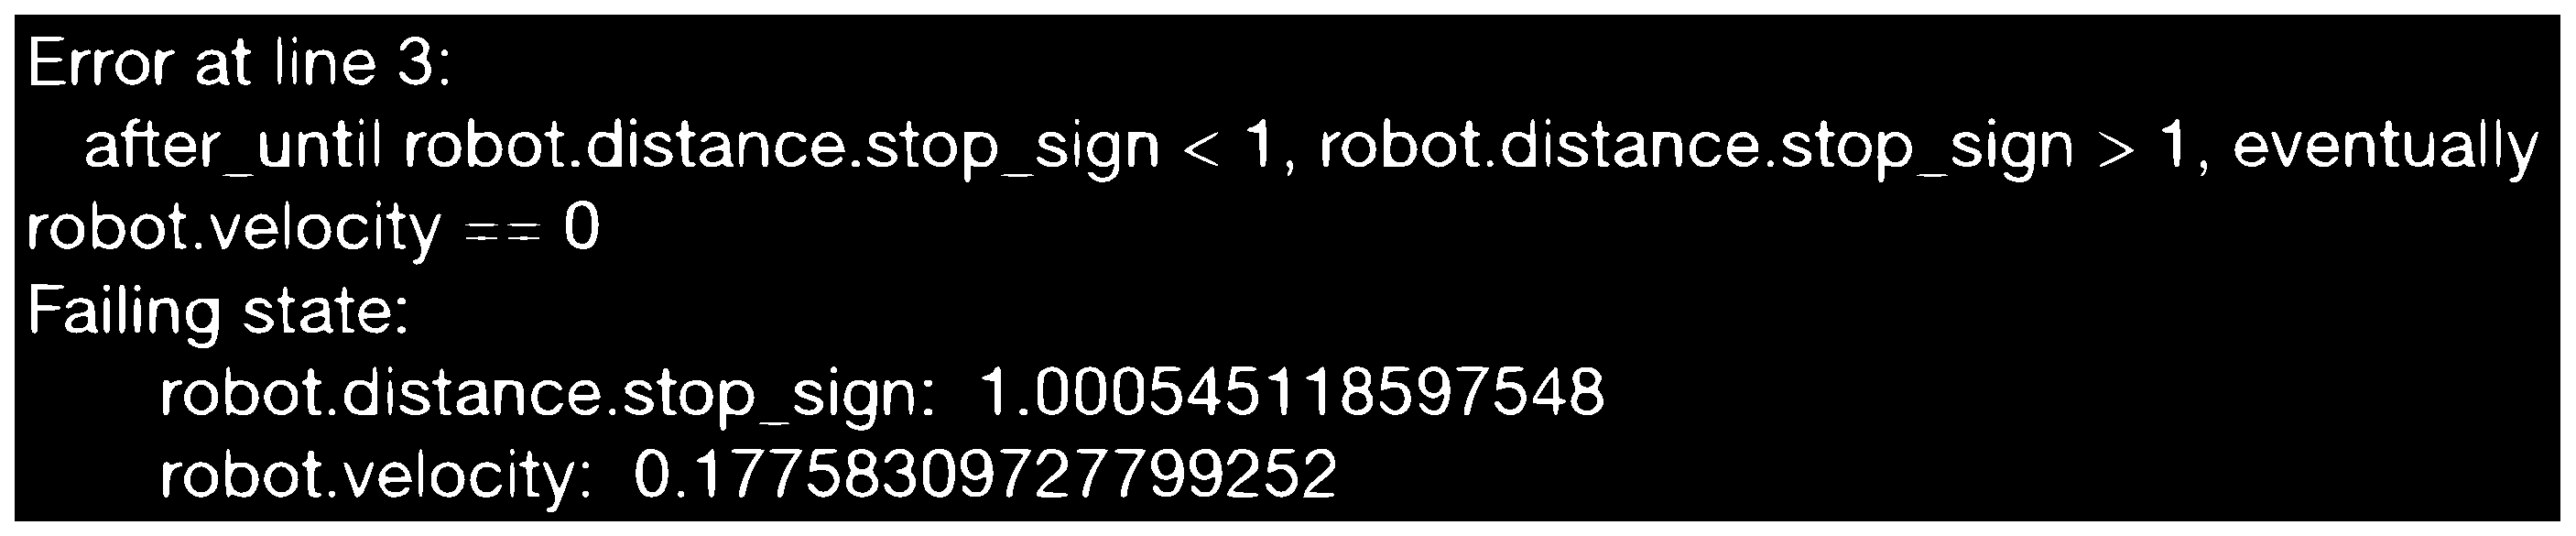
\includegraphics[width=\textwidth]{error.eps}
\caption{Example of the displayed error when the robot doesn't stop at the stop sign.} \label{fig1}
\end{figure}

The whole flow of the process of monitoring a robotic system is below enumerated:

\begin{enumerate}[label=(\roman*)]
    \item Using the DSL write the properties of the robotic system one wants to monitor in a .txt file extension
    \item The specified properties are compiled and a python file is generated which is capable of running as a ROS node
    \item The node can be run whenever testing the system and will listen to relevant topics and perform the computations needed to verify the specified properties.
\end{enumerate}


\section{Specification Language for Robotics Properties}

The domain-specific language relies on an adaptation of LTL to express temporal relations of and between simulation objects. The domain-specific language also has shortcuts to express the absolute values of certain useful concepts of objects in a simulation.

\subsection{Temporal Keywords}

We consider not only LTL basic operators but also some common shortcuts for useful combinations of such operators, like \textit{after\_until}, used in the example:

\begin{itemize}
\item {\bfseries always X} - X has to hold on the entire subsequent path;
\item {\bfseries never X} - X never holds on the entire subsequent path;
\item {\bfseries eventually X} - X eventually has to hold, somewhere on the subsequent path;
\item {\bfseries after X, Y} - after the event X is observed, Y has to hold on the entire subsequent path;
\item {\bfseries until X, Y} - X holds at the current or future position, and Y has to hold until that position. At that position, Y does not have to hold anymore;
\item {\bfseries after\_until X, Y, Z} - after the event X is observed, Z has to hold on the entire subsequent path up until Y happens, at that position Z does not have to hold anymore;
\end{itemize}

\noindent It is also possible to reference previous states of variables, using \lstinline|@{X, -y}|, representing the value of variable \lstinline|X| at time \lstinline|-y|.

\subsection{Simulation primivitives}

To support comparing the internal state of the robotic system with the environment, we provide basic primitives in the language to refer to the simulation environment:

\begin{itemize}
\item {\bfseries X.position} - The position of the robot in the simulation;
\item {\bfseries X.position.y} - The position in the y axis of the robot in the simulation. Also works for x and z;
\item {\bfseries X.distance.Y} - The absolute distance between two objects in the simulation. For the x and y axis;
\item {\bfseries X.distanceZ.Y} - The absolute distance between two objects in the simulation. For the x, y, and z axis;
\item {\bfseries X.velocity} - The velocity of an object in the simulation. This refers to linear velocity;
\item {\bfseries X.velocity.x} - The velocity in the x axis of an object in the simulation. This refers to linear velocity;
\item {\bfseries X.localization\_error} - The difference between the robot's perception of its position and the actual position in the simulation;
\end{itemize}


\subsection{Topic declaration}

In order to relate robot components with the simulation, the developer can declare the relevant \textit{topic}.

\textit{The variable robot\_position was declared with the type Odometry.pose.pose.position and is linked to the topic /odom;}

\vspace{3mm}

\texttt{decl robot\_position /odom Odometry.pose.pose.position}


\subsection{Model robots}

There are a set of specific topics that can be modeled for the robot, like \textit{position} or \textit{velocity}. These will be used by the compiler to call specific functions that need this information from the robot's perspective.

\vspace{3mm}

\texttt{model robot1:}

\texttt{    position /odom Odometry.pose.pose.position}

\texttt{    ;}

\vspace{3mm}

\texttt{never robot1.localization error > 0.002}


\section{Examples}

To validate the expressive power of our language, we present examples of expressions, inspired by real-world scenarios.


\subsection{Vehicle Maximum Speed}

Some robots have a maximum safe speed at which they can move. Sometimes this limit is imposed by law, but some other times by physical constraints.


\textit{The robot velocity will never be above 2 for the duration of the simulation;}

\vspace{3mm}

\texttt{never robot.velocity > 2.0}

\subsection{Follow the Leader}

The first robot being above 1 velocity implies that the second robot is at least at 0.8 distance from the first robot. Up until they reach a certain location;

\vspace{3mm}

\texttt{until (robot1.position.x > 45 and robot1.position.y > 45), always (robot1.velocity > 1 implies robot2.distance.robot1 > 0.8)}


\subsection{Drone height rotors control}

After a drone is at a certain altitude both rotors always have the same velocity up until the drone decreases to a certain altitude

\vspace{3mm}

\texttt{decl rotor1\_vel /drone\_mov/rotor1 Vector3.linear.x}

\texttt{decl rotor2\_vel /drone\_mov/rotor2 Vector3.linear.x}

\vspace{3mm}

\texttt{after\_until drone.position.z > 5, drone.position.z < 5, rotor1\_vel == rotor2\_vel}


\section{Related work}

% https://link.springer.com/chapter/10.1007/978-3-319-11164-3_20

% https://link.springer.com/chapter/10.1007/978-3-030-63486-5_40

% https://link.springer.com/book/10.1007/978-3-319-67531-2?noAccess=true

% https://www.human-competitive.org/sites/default/files/a_search-based_framework_for_automatic_generation_of_testing_environments_0.pdf

% https://clairelegoues.com/papers/zizyte21dsn.pdf

% https://rose-workshops.github.io/files/rose2022/papers/RoSE22_paper_4.pdf

\section{Conclusion}

The proposed approach is capable of expressing some interesting scenarios that developers care about. We are in the process of expanding our examples to include bugs found in real work projects~\cite{robust_repo} and from a survey we are conducting with expert developers.

Our development is available online~\cite{github_repo}, for those that want to experiment with it. We also intend on expanding the primitives with more simulator information, or with the possibility of integrating sensors for supporting field testing in alternative to simulation.


\begin{thebibliography}{8}
%\bibitem{ref_article1}
%Author, F.: Article title. Journal \textbf{2}(5), 99--110 (2016)

%\bibitem{ref_lncs1}
%Author, F., Author, S.: Title of a proceedings paper. In: Editor,
%F., Editor, S. (eds.) CONFERENCE 2016, LNCS, vol. 9999, pp. 1--13.
%Springer, Heidelberg (2016). \doi{10.10007/1234567890}

\bibitem{robust_repo}
GitHub repository of ROBUST: ROS Bug Study, \url{https://github.com/robust-rosin/robust}

\bibitem{github_repo}
GitHub repository of our work, \url{https://ricardocajo.github.io/error-monitor-ros-gazebo}
\end{thebibliography}
\end{document}
